\documentclass{article}

% content/resources/templates/preamble.tex
\usepackage[margin=0.6in]{geometry}
\author{Milav Dabgar}
\usepackage{amsmath,amssymb,amsthm}
\usepackage{booktabs}
\usepackage{multirow}
\usepackage{xcolor}
\usepackage{tcolorbox}
\tcbuselibrary{breakable,skins}
\usepackage[colorlinks=true,linkcolor=blue]{hyperref}
\usepackage{titlesec}
\usepackage{enumitem}
\usepackage{tikz}
\usepackage{pgfplots}
\usepackage{circuitikz}
\usepackage[version=4]{mhchem}
\usepackage{longtable}
\usepackage{array}
\usepackage{float}
\usepackage{caption}
\usepackage{listings}

\lstset{
  basicstyle=\small\ttfamily,
  breaklines=true,
  breakatwhitespace=false,
  postbreak=\mbox{\textcolor{red}{$\hookrightarrow$}\space},
  float=false,
  numbers=left,
  numberstyle=\tiny\color{gray},
  numbersep=10pt,
  xleftmargin=2em,
  keywordstyle=\color{blue},
  commentstyle=\color{green!60!black},
  stringstyle=\color{purple},
  backgroundcolor=\color{gray!5},
  showstringspaces=false,
  tabsize=2,
  captionpos=b,
  keepspaces=true,
  columns=flexible
}

\pgfplotsset{compat=1.18}
\usetikzlibrary{shapes,arrows,positioning,calc,patterns,decorations.pathmorphing,decorations.markings,arrows.meta}

% Color scheme
\definecolor{headcolor}{RGB}{0,102,204}
\definecolor{keycolor}{RGB}{220,20,60}
\definecolor{solutioncolor}{RGB}{34,139,34}
\definecolor{mnemoniccolor}{RGB}{148,0,211}
\definecolor{codecolor}{RGB}{0,0,100}

% Spacing
\setlength{\parskip}{3pt}
\setlist[itemize]{nosep}
\setlist[enumerate]{nosep}

% Title formatting
\titleformat{\section}{\Large\bfseries\color{headcolor}}{\thesection}{1em}{}
\titleformat{\subsection}{\large\bfseries\color{headcolor}}{\thesubsection}{1em}{}

% Pandoc tightlist compatibility
\providecommand{\tightlist}{%
  \setlength{\itemsep}{0pt}\setlength{\parskip}{0pt}}

% Pandoc longtable compatibility
\newcounter{none}
\def\thenone{}


% content/resources/templates/english-boxes.tex

% Custom environments
\newtcolorbox{solutionbox}{
 breakable,
 enhanced,
 colback=solutioncolor!5!white,
 colframe=solutioncolor!75!black,
 fonttitle=\bfseries,
 title=Solution
}

\newtcolorbox{solutionboxnobreak}{
 colback=solutioncolor!5!white,
 colframe=solutioncolor!75!black,
 fonttitle=\bfseries,
 title=Solution
}

\newtcolorbox{keyformula}{
 breakable,
 enhanced,
 colback=keycolor!5!white,
 colframe=keycolor!75!black,
 fonttitle=\bfseries,
 title=Key Formula
}

\newtcolorbox{mnemonicboxenv}{
 breakable,
 enhanced,
 colback=mnemoniccolor!5!white,
 colframe=mnemoniccolor!75!black,
 fonttitle=\bfseries,
 title=Mnemonic
}

\newcommand{\mnemonicbox}[1]{%
  \begin{mnemonicboxenv}
    #1
  \end{mnemonicboxenv}
}


% Custom commands for GTU solutions
% This file defines semantic commands for consistent formatting

% Question command with automatic formatting
\newcommand{\question}[2]{%
  \section*{Question #1}%
  \textbf{#2}%
}

% OR question variant
\newcommand{\questionor}[2]{%
  \section*{Question #1 OR}%
  \textbf{#2}%
}

% Proper table environment with caption
\newenvironment{answertable}[1]{%
  \begin{table}[htbp]
  \centering
  \caption{#1}
}{%
  \end{table}
}

% Proper figure environment for diagrams
\newenvironment{answerdiagram}[1]{%
  \begin{figure}[htbp]
  \centering
  \caption{#1}
}{%
  \end{figure}
}

% Semantic markup for key terms
\newcommand{\keyword}[1]{\textbf{#1}}
\newcommand{\code}[1]{\texttt{#1}}
\newcommand{\classname}[1]{\texttt{#1}}
\newcommand{\methodname}[1]{\texttt{#1}}

% Proper quotation marks
\newcommand{\mnemonic}[1]{``#1''}


\title{Electronic Measurements \& Instruments (4331102) - Winter 2024 Solution}
\date{December 05, 2024}

\begin{document}
\maketitle

\questionmarks{1(a)}{3}{Define following term: (1) Accuracy (2) Resolution (3) Error}

\begin{solutionbox}
\begin{center}
\captionof{table}{Definitions}
\begin{tabulary}{\linewidth}{|L|L|}
\hline
\textbf{Term} & \textbf{Definition} \\ \hline
\textbf{Accuracy} & The closeness of a measurement to the true value \\ \hline
\textbf{Resolution} & The smallest change in input that can be detected by an instrument \\ \hline
\textbf{Error} & The difference between measured value and true value \\ \hline
\end{tabulary}
\end{center}
\end{solutionbox}

\begin{mnemonicbox}
\mnemonic{ARE precise: Accuracy shows Reality, Error shows deviation, Resolution shows detail.}
\end{mnemonicbox}

\questionmarks{1(b)}{4}{Explain construction of unbounded strain gauge transducer with necessary diagram in detail. Also list application of it.}

\begin{solutionbox}
An unbounded strain gauge consists of a fine wire wound in a grid pattern attached to a backing material.

\begin{center}
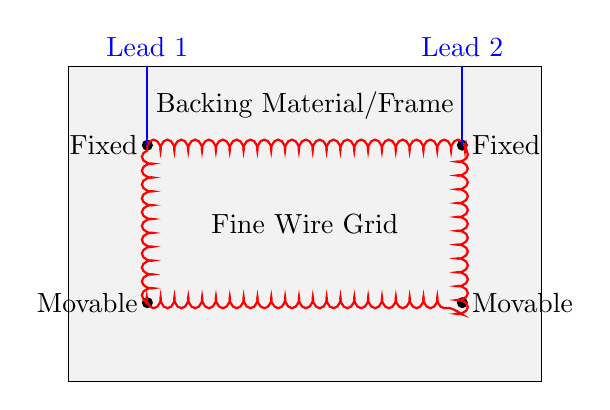
\begin{tikzpicture}
    % Frame
    \draw[fill=gray!10] (0,0) rectangle (6,4);
    \node at (3,3.5) {Backing Material/Frame};
    
    % Pins
    \foreach \x in {1, 5} \foreach \y in {1, 3} \fill (\x,\y) circle (2pt);
    \node[left] at (1,3) {Fixed}; \node[right] at (5,3) {Fixed};
    \node[left] at (1,1) {Movable}; \node[right] at (5,1) {Movable};
    
    % Wire
    \draw[thick, red, decorate, decoration={coil, amplitude=2pt, segment length=5pt}] (1,3) -- (5,3) -- (5,1) -- (1,1) -- (1,3);
    \node at (3,2) [align=center] {Fine Wire Grid};
    
    % Leads
    \draw[thick, blue] (1,3) -- (1,4) node[above] {Lead 1};
    \draw[thick, blue] (5,3) -- (5,4) node[above] {Lead 2};
\end{tikzpicture}
\captionof{figure}{Unbounded Strain Gauge}
\end{center}

\begin{itemize}
    \item \textbf{Construction elements}: Fine resistance wire is looped back and forth on an insulating base material
    \item \textbf{Working principle}: Changes resistance when subjected to strain
    \item \textbf{Applications}: Weight measurement, pressure sensors, force sensors, structural health monitoring
\end{itemize}
\end{solutionbox}

\begin{mnemonicbox}
\mnemonic{WIRE Flexes: Wire grids Indicate Resistance changes from External stress.}
\end{mnemonicbox}

\questionmarks{1(c)}{7}{Explain working of Schering Bridge with circuit diagram for balance condition. List its advantages, disadvantages and applications.}

\begin{solutionbox}
Schering Bridge is an AC bridge used to measure unknown capacitance and its dissipation factor.

\begin{center}
\begin{circuitikz}[american, scale=0.8]
    \draw (0,3) to[C, l=$C_x$] (3,5) node[above] {B} to[C, l=$C_2$] (6,3) node[right] {C};
    \draw (6,3) to[R, l=$R_2$] (3,1) node[below] {D};
    \draw (3,1) to[R, l=$R_1$] (0,3);
    \draw (3,5) to[rmeter, t=D] (3,1);
    \draw (0,3) -- (-1,3) to[sV, l=AC] (-1,1) -- (3,1);
\end{circuitikz}
\captionof{figure}{Schering Bridge}
\end{center}

\textbf{Balance condition:}

\begin{center}
\captionof{table}{Balance Condition}
\begin{tabulary}{\linewidth}{|L|L|}
\hline
\textbf{Equation} & \textbf{Description} \\ \hline
$C_x = C_2(R_2/R_1)$ & For capacitance calculation \\ \hline
$D_x = R_2(C_2/C_x)$ & For dissipation factor \\ \hline
\end{tabulary}
\end{center}

\textbf{Advantages:}
\begin{itemize}
    \item High accuracy
    \item Direct reading of capacitance
    \item Wide measurement range
\end{itemize}

\textbf{Disadvantages:}
\begin{itemize}
    \item Requires careful shielding
    \item Frequency dependent errors
    \item Complex to balance
\end{itemize}

\textbf{Applications:}
\begin{itemize}
    \item Capacitor testing
    \item Insulation testing
    \item Dielectric material evaluation
\end{itemize}
\end{solutionbox}

\begin{mnemonicbox}
\mnemonic{SCUBA dive: Schering Calculates Unknown capacitance By Advanced circuit Designs In Various Equipment.}
\end{mnemonicbox}

\questionmarks{1(c) OR}{7}{Explain working of Maxwell's bridge with circuit diagram for balance condition. List its advantages, disadvantages, and applications.}

\begin{solutionbox}
Maxwell's bridge is used to measure unknown inductance in terms of known capacitance.

\begin{center}
\begin{circuitikz}[american, scale=0.8]
    \draw (0,3) node[left] {A} to[R, l=$R_1$] (3,6) node[above] {B} to[R, l=$R_3$] (6,3) node[right] {C};
    \draw (6,3) to[R, l=$R_2$] (6,1.5) -- (3,0) node[below] {D};
    \draw (6,3) -- (6,4) to[C, l=$C_4$] (3,0);
    \draw (0,3) to[L, l=$L_x$] (1.5,1.5) to[R, l=$R_x$] (3,0);
    \draw (3,6) to[rmeter, t=D] (3,0);
    \draw (0,3) -- (-1,3) to[sV, l=AC] (-1,0) -- (3,0);
\end{circuitikz}
\captionof{figure}{Maxwell's Bridge}
\end{center}

\textbf{Balance condition:}

\begin{center}
\captionof{table}{Balance Condition}
\begin{tabulary}{\linewidth}{|L|L|}
\hline
\textbf{Equation} & \textbf{Description} \\ \hline
$L_x = C_4 \cdot R_2 \cdot R_3$ & For inductance calculation \\ \hline
$R_x = R_1 \cdot (R_3/R_2)$ & For resistance calculation \\ \hline
\end{tabulary}
\end{center}

\textbf{Advantages:}
\begin{itemize}
    \item Independent of frequency
    \item High accuracy for medium Q coils
    \item Easy to balance
\end{itemize}

\textbf{Disadvantages:}
\begin{itemize}
    \item Not suitable for low Q coils
    \item Requires standard capacitor
    \item Limited range
\end{itemize}

\textbf{Applications:}
\begin{itemize}
    \item Measuring inductors
    \item Audio frequency measurements
    \item Transformer testing
\end{itemize}
\end{solutionbox}

\begin{mnemonicbox}
\mnemonic{MAGIC bridge: Maxwell Analyses Great Inductors by Comparing bridge Elements.}
\end{mnemonicbox}

\questionmarks{2(a)}{3}{Explain working of electronic multimeter with necessary diagram.}

\begin{solutionbox}
Electronic multimeter converts various electrical parameters into proportional DC voltage for measurement.

\begin{center}
\begin{tikzpicture}[node distance=1.5cm, auto, scale=0.8, every node/.style={transform shape}]
    \node [gtu block] (Input) {Input Selection};
    \node [gtu block, right=of Input] (Atten) {Attenuator/Range Selector};
    \node [gtu block, right=of Atten] (Conv) {Converter Circuit};
    \node [gtu block, below=of Conv] (Amp) {Amplifier};
    \node [gtu block, left=of Amp] (ADC) {ADC};
    \node [gtu block, left=of ADC] (Disp) {Display};

    \draw [gtu arrow] (Input) -- (Atten);
    \draw [gtu arrow] (Atten) -- (Conv);
    \draw [gtu arrow] (Conv) -- (Amp);
    \draw [gtu arrow] (Amp) -- (ADC);
    \draw [gtu arrow] (ADC) -- (Disp);
\end{tikzpicture}
\captionof{figure}{Electronic Multimeter Block Diagram}
\end{center}

\begin{itemize}
    \item \textbf{Circuit elements}: Input selector $\to$ Attenuator $\to$ Converter $\to$ Amplifier $\to$ ADC $\to$ Display
    \item \textbf{Measurement types}: DC voltage, AC voltage, Current, Resistance
    \item \textbf{Power source}: Battery powered for portability and safety
\end{itemize}
\end{solutionbox}

\begin{mnemonicbox}
\mnemonic{SACRED device: Signal Attenuated, Converted And Rectified for Electronic Display.}
\end{mnemonicbox}

\questionmarks{2(b)}{4}{Differentiate between Digital Voltmeter over Analog Voltmeter.}

\begin{solutionbox}
\begin{center}
\captionof{table}{Differentiation}
\begin{tabulary}{\linewidth}{|L|L|L|}
\hline
\textbf{Parameter} & \textbf{Digital Voltmeter} & \textbf{Analog Voltmeter} \\ \hline
\textbf{Display type} & Numeric LCD/LED display & Moving pointer on scale \\ \hline
\textbf{Accuracy} & Higher ($\pm 0.1\%$ typical) & Lower ($\pm 2-5\%$ typical) \\ \hline
\textbf{Reading errors} & No parallax error & Prone to parallax error \\ \hline
\textbf{Resolution} & Higher (can display 3-6 digits) & Limited by scale divisions \\ \hline
\textbf{Input impedance} & Very high ($>10M\Omega$) & Lower ($20-200k\Omega/V$) \\ \hline
\textbf{Response time} & Slower sampling rate & Instant response \\ \hline
\end{tabulary}
\end{center}
\end{solutionbox}

\begin{mnemonicbox}
\mnemonic{PARIOS: Parallax-free, Accurate, Resolution high, Impedance high, Observation digital, Sampling rate.}
\end{mnemonicbox}

\questionmarks{2(c)}{7}{Describe construction diagram of Energy meter and explain in detail.}

\begin{solutionbox}
Energy meter measures electrical energy consumption over time in kilowatt-hours (kWh).

\begin{center}
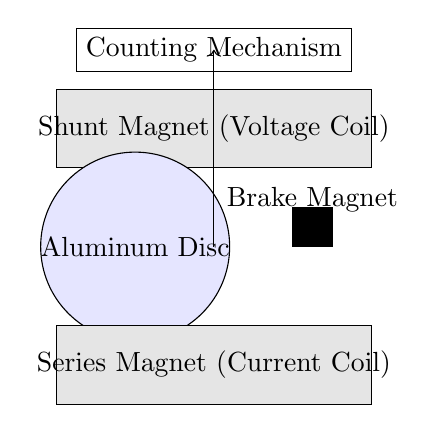
\begin{tikzpicture}
    % Construction
    \draw[fill=gray!20] (0,3) rectangle (4,4); \node at (2,3.5) {Shunt Magnet (Voltage Coil)};
    \draw[fill=blue!10] (1,2) circle (1.2); \node at (1,2) {Aluminum Disc};
    \draw[fill=gray!20] (0,0) rectangle (4,1); \node at (2,0.5) {Series Magnet (Current Coil)};
    \draw[fill=black] (3,2) rectangle (3.5, 2.5); \node at (3.25, 2.6) {Brake Magnet};
    \node[draw] at (2, 4.5) {Counting Mechanism};
    \draw [->] (2, 2) -- (2, 4.5);
\end{tikzpicture}
\captionof{figure}{Energy Meter Construction}
\end{center}

\textbf{Components:}
\begin{itemize}
    \item \textbf{Voltage coil}: Creates flux proportional to voltage
    \item \textbf{Current coil}: Creates flux proportional to current
    \item \textbf{Aluminum disc}: Rotates due to eddy currents
    \item \textbf{Counting mechanism}: Registers disc rotations
    \item \textbf{Permanent magnet}: Acts as brake to control disc speed
    \item \textbf{Adjustment systems}: For calibration and accuracy
\end{itemize}

\textbf{Working principle}: Disc rotation speed is proportional to power consumption ($V \times I \times \cos\Phi$)
\end{solutionbox}

\begin{mnemonicbox}
\mnemonic{VADCR meter: Voltage And current Drive Counter through Rotations.}
\end{mnemonicbox}

\questionmarks{2(a) OR}{3}{Explain working of clamp on Ammeter with necessary diagram.}

\begin{solutionbox}
Clamp-on ammeter measures current without breaking the circuit by using electromagnetic induction.

\begin{center}
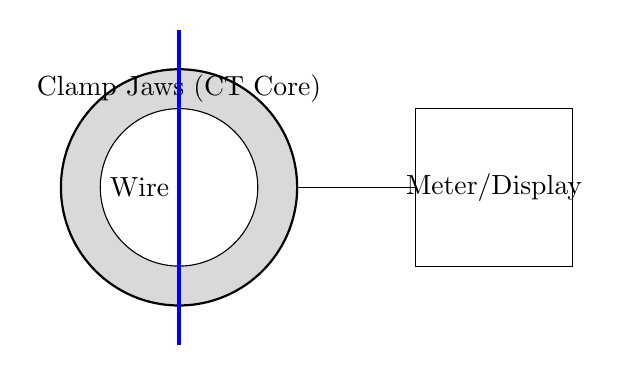
\begin{tikzpicture}
    \draw[thick, fill=gray!30] (0,0) circle (1.5); \draw[fill=white] (0,0) circle (1);
    \node at (0, 1.25) {Clamp Jaws (CT Core)};
    \draw[ultra thick, blue] (0, -2) -- (0, 2); \node[left] at (0, 0) {Wire};
    \draw (1.5, 0) -- (3, 0); \draw (3, -1) rectangle (5, 1); \node at (4, 0) {Meter/Display};
\end{tikzpicture}
\captionof{figure}{Clamp-on Ammeter}
\end{center}

\begin{itemize}
    \item \textbf{Construction}: Split ferrite core with sensing coil
    \item \textbf{Working principle}: Current-carrying wire creates magnetic field $\to$ induces voltage in sensing coil
    \item \textbf{Advantages}: Non-contact measurement, quick, safe
\end{itemize}
\end{solutionbox}

\begin{mnemonicbox}
\mnemonic{CICS: Clamping Induces Current Signal.}
\end{mnemonicbox}

\questionmarks{2(b) OR}{4}{Differentiate between PMMC type Meter over Moving iron type Meter.}

\begin{solutionbox}
\begin{center}
\captionof{table}{PMMC vs Moving Iron}
\begin{tabulary}{\linewidth}{|L|L|L|}
\hline
\textbf{Parameter} & \textbf{PMMC Type Meter} & \textbf{Moving Iron Type Meter} \\ \hline
\textbf{Operating principle} & Magnetic field interaction & Magnetic attraction/repulsion \\ \hline
\textbf{Current type} & DC only & Both AC and DC \\ \hline
\textbf{Scale} & Uniform & Non-uniform (crowded at ends) \\ \hline
\textbf{Accuracy} & Higher ($\pm 0.5\%$ typical) & Lower ($\pm 1-5\%$ typical) \\ \hline
\textbf{Damping} & Eddy current damping & Air friction damping \\ \hline
\textbf{Power consumption} & Low & High \\ \hline
\textbf{Frequency errors} & Not applicable & Affected by frequency changes \\ \hline
\end{tabulary}
\end{center}
\end{solutionbox}

\begin{mnemonicbox}
\mnemonic{PMMC is DAUPHIN: DC only, Accurate, Uniform scale, Power efficient, High sensitivity, Independent of frequency, Needs polarity.}
\end{mnemonicbox}

\questionmarks{2(c) OR}{7}{Draw the block diagram and Explain working of Integrating type DVM with necessary diagram and waveform.}

\begin{solutionbox}
Integrating type DVM converts input voltage to time through integration for high accuracy measurements.

\begin{center}
\begin{tikzpicture}[node distance=1.5cm, auto, scale=0.8, every node/.style={transform shape}]
    \node [gtu block] (Buffer) {Input Buffer};
    \node [gtu block, right=of Buffer] (Integrator) {Integrator};
    \node [gtu block, right=of Integrator] (Comparator) {Comparator};
    \node [gtu block, below=of Comparator] (Logic) {Control Logic};
    \node [gtu block, right=of Logic] (Counter) {Counter};
    \node [gtu block, right=of Counter] (Display) {Display};
    \node [gtu block, below=of Logic] (Clock) {Clock};

    \draw [gtu arrow] (Buffer) -- (Integrator);
    \draw [gtu arrow] (Integrator) -- (Comparator);
    \draw [gtu arrow] (Comparator) -- (Logic);
    \draw [gtu arrow] (Logic) -- (Counter);
    \draw [gtu arrow] (Counter) -- (Display);
    \draw [gtu arrow] (Clock) -- (Logic);
    \draw [gtu arrow] (Logic) -| (Integrator) node[midway, above] {Reset};
\end{tikzpicture}
\captionof{figure}{Integrating DVM Block Diagram}
\end{center}

\textbf{Working principle:}
\begin{itemize}
    \item Input voltage is integrated for fixed time period
    \item Integrator output ramps up proportionally to input
    \item Reference voltage with opposite polarity discharges integrator
    \item Time taken for discharge is measured by counting clock pulses
    \item Count is proportional to input voltage
\end{itemize}

\textbf{Waveforms:}
\begin{center}
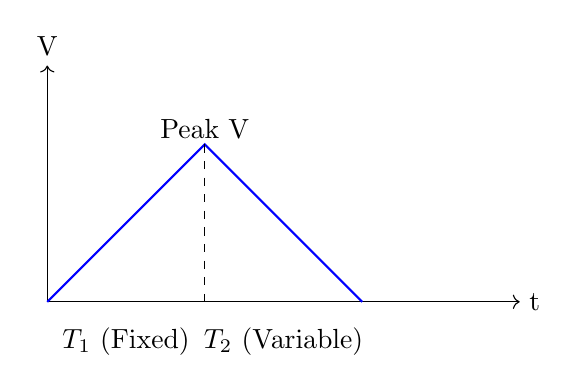
\begin{tikzpicture}
    \draw[->] (0,0) -- (6,0) node[right] {t};
    \draw[->] (0,0) -- (0,3) node[above] {V};
    \draw[thick, blue] (0,0) -- (2,2) -- (4,0);
    \node at (1, -0.5) {$T_1$ (Fixed)};
    \node at (3, -0.5) {$T_2$ (Variable)};
    \draw[dashed] (2,2) -- (2,0);
    \node at (2, 2.2) {Peak V};
\end{tikzpicture}
\captionof{figure}{Integration Waveform}
\end{center}
\end{solutionbox}

\begin{mnemonicbox}
\mnemonic{DIRT meter: Direct Integration Relates Time to measure voltage.}
\end{mnemonicbox}

\questionmarks{3(a)}{3}{Differentiate between CRO over DSO.}

\begin{solutionbox}
\begin{center}
\captionof{table}{CRO vs DSO}
\begin{tabulary}{\linewidth}{|L|L|L|}
\hline
\textbf{Parameter} & \textbf{CRO (Analog Oscilloscope)} & \textbf{DSO (Digital Storage Oscilloscope)} \\ \hline
\textbf{Signal processing} & Analog throughout & Digital after ADC conversion \\ \hline
\textbf{Storage capability} & Cannot store waveforms & Can store multiple waveforms \\ \hline
\textbf{Bandwidth} & Typically lower & Higher (can exceed GHz) \\ \hline
\textbf{Triggering} & Basic trigger options & Advanced trigger capabilities \\ \hline
\textbf{Analysis features} & Limited & Extensive (FFT, measurements) \\ \hline
\textbf{Display persistence} & Phosphor persistence & Adjustable digital persistence \\ \hline
\end{tabulary}
\end{center}
\end{solutionbox}

\begin{mnemonicbox}
\mnemonic{PASSED: Processing-Analog/digital, Storage-none/yes, Signal-raw/processed, Easy-basic/advanced, Display-phosphor/digital.}
\end{mnemonicbox}

\questionmarks{3(b)}{4}{Explain CRO Screen.}

\begin{solutionbox}
CRO screen displays electrical signals and consists of several important elements.

\begin{center}
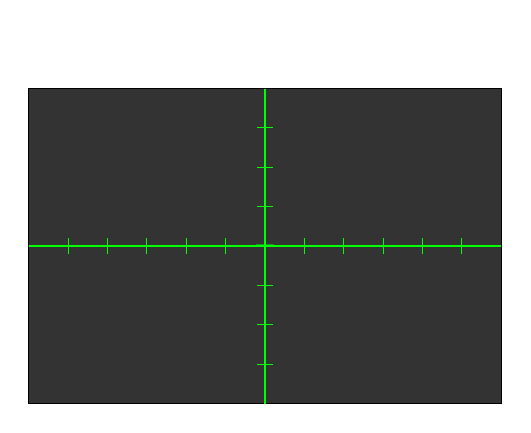
\begin{tikzpicture}
    \draw[fill=black!80] (0,0) rectangle (6,4);
    \draw[green, thick] (0,2) -- (6,2);
    \draw[green, thick] (3,0) -- (3,4);
    \foreach \x in {0.5,1,...,5.5} \draw[green] (\x,1.9) -- (\x,2.1);
    \foreach \y in {0.5,1,...,3.5} \draw[green] (2.9,\y) -- (3.1,\y);
    \node[green] at (3,2) {+};
    \node[white] at (3, 4.5) {Phosphor Screen};
\end{tikzpicture}
\captionof{figure}{CRO Screen Graticule}
\end{center}

\textbf{Components:}
\begin{itemize}
    \item \textbf{Phosphor coating}: Emits light when struck by electrons
    \item \textbf{Graticule}: Grid lines for measurement reference
    \item \textbf{Scales}: Calibrated markings for voltage/time
    \item \textbf{Center reference point}: (0,0) coordinate
    \item \textbf{Intensity control}: Adjusts brightness of display
\end{itemize}
\end{solutionbox}

\begin{mnemonicbox}
\mnemonic{PGSCR: Phosphor Glows when Struck, Creating Representation.}
\end{mnemonicbox}

\questionmarks{3(c)}{7}{Explain Block diagram, working and advantage of CRO with necessary diagram.}

\begin{solutionbox}
CRO (Cathode Ray Oscilloscope) visualizes electrical signals as waveforms.

\begin{center}
\begin{tikzpicture}[node distance=1.2cm, auto, scale=0.7, every node/.style={transform shape}]
    \node [gtu block] (Input) {Vertical Input};
    \node [gtu block, right=of Input] (Atten) {Vert. Attenuator};
    \node [gtu block, right=of Atten] (Amp) {Vert. Amp};
    \node [gtu block, right=of Amp] (PlatesV) {Vertical Plates};
    \node [gtu block, below=of Input] (Trig) {Trigger Circuit};
    \node [gtu block, right=of Trig] (TimeBase) {Time Base};
    \node [gtu block, right=of TimeBase] (HorAmp) {Horiz. Amp};
    \node [gtu block, right=of HorAmp] (PlatesH) {Horiz. Plates};
    \node [gtu block, below=of Trig] (Power) {Power Supply};
    \node [gtu block, right=of Power] (Gun) {Electron Gun};
    \node [circle, draw, minimum size=1cm, right=of PlatesV] (CRT) {CRT};

    \draw [gtu arrow] (Input) -- (Atten);
    \draw [gtu arrow] (Atten) -- (Amp);
    \draw [gtu arrow] (Amp) -- (PlatesV);
    \draw [gtu arrow] (Trig) -- (TimeBase);
    \draw [gtu arrow] (TimeBase) -- (HorAmp);
    \draw [gtu arrow] (HorAmp) -- (PlatesH);
    \draw [gtu arrow] (Power) -- (Gun);
    \draw [gtu arrow] (Gun) -| (CRT);
    \draw [gtu arrow] (PlatesV) -- (CRT);
    \draw [gtu arrow] (PlatesH) -- (CRT);
\end{tikzpicture}
\captionof{figure}{CRO Block Diagram}
\end{center}

\textbf{Working principle:}
\begin{itemize}
    \item \textbf{Electron gun}: Generates electron beam
    \item \textbf{Vertical system}: Controls Y-axis deflection proportional to input signal
    \item \textbf{Horizontal system}: Sweeps beam across screen at constant rate
    \item \textbf{Trigger circuit}: Synchronizes horizontal sweep with input signal
    \item \textbf{CRT}: Displays electron beam movement on phosphor screen
\end{itemize}

\textbf{Advantages:}
\begin{itemize}
    \item Real-time signal display
    \item Wide bandwidth
    \item High input impedance
    \item Versatile triggering options
    \item Multiple signal analysis
\end{itemize}
\end{solutionbox}

\begin{mnemonicbox}
\mnemonic{EARTH view: Electron beam Amplification Reveals Time-based Horizontal view.}
\end{mnemonicbox}


\questionmarks{3(a) OR}{3}{Apply Lissajous pattern for frequency measurement and Phase angle measurement.}

\begin{solutionbox}
Lissajous patterns are created when two sine waves are applied to X and Y inputs of CRO.

\begin{center}
\captionof{table}{Lissajous Measurements}
\begin{tabulary}{\linewidth}{|L|L|L|}
\hline
\textbf{Pattern Type} & \textbf{Measurement Formula} \\ \hline
\textbf{Frequency Measurement} & $f_x/f_y = n_y/n_x$ (Tangent ratio) \\ \hline
\textbf{Phase Angle Measurement} & $\sin(\phi) = A/B$ (Intercept/Max Height) \\ \hline
\end{tabulary}
\end{center}

\begin{center}
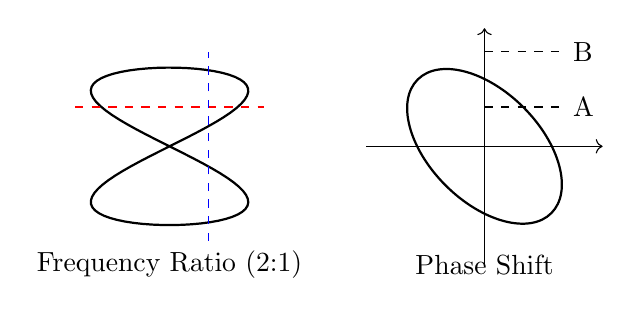
\begin{tikzpicture}
    % Frequency (2:1)
    \begin{scope}[shift={(0,0)}]
        \draw[thick, samples=100, domain=0:2*pi] plot ({sin(2*\x r)}, {sin(\x r)});
        \node at (0, -1.5) {Frequency Ratio (2:1)};
        \draw[red, dashed] (-1.2, 0.5) -- (1.2, 0.5); 
        \draw[blue, dashed] (0.5, -1.2) -- (0.5, 1.2);
    \end{scope}
    
    % Phase
    \begin{scope}[shift={(4,0)}]
        \draw[thick, rotate=45] (0,0) ellipse (0.7 and 1.2);
        \draw[->] (-1.5,0) -- (1.5,0);
        \draw[->] (0,-1.5) -- (0,1.5);
        \node at (0, -1.5) {Phase Shift};
        \draw[dashed] (0, 0.5) -- (1, 0.5) node[right] {A};
        \draw[dashed] (0, 1.2) -- (1, 1.2) node[right] {B};
    \end{scope}
\end{tikzpicture}
\captionof{figure}{Lissajous Patterns}
\end{center}

\begin{itemize}
    \item \textbf{Frequency ratio}: Count vertical tangent points / horizontal tangent points
    \item \textbf{Phase measurement}: $\sin(\phi) = A/B$ where A is pattern height at zero crossing, B is max height
    \item \textbf{Applications}: Signal comparison, frequency calibration
\end{itemize}
\end{solutionbox}

\begin{mnemonicbox}
\mnemonic{LIPS patterns: Lissajous Indicates Phase and Sine frequency.}
\end{mnemonicbox}

\questionmarks{3(b) OR}{4}{Explain Graticules in CRO. Also Explain its types.}

\begin{solutionbox}
Graticules are reference grids on a CRO screen that help in measurement of waveform parameters.

\begin{center}

\begin{tikzpicture}
    \draw[step=1cm, gray!50, thin] (0,0) grid (6,4);
    \draw[thick] (0,0) rectangle (6,4);
    \draw[thick] (3,0) -- (3,4);
    \draw[thick] (0,2) -- (6,2);
    \foreach \x in {0,1,2,3,4,5,6} \draw (\x, 1.9) -- (\x, 2.1);
    \foreach \y in {0,1,2,3,4} \draw (2.9, \y) -- (3.1, \y);
\end{tikzpicture}
\captionof{figure}{CRO Graticule}
\end{center}

\textbf{Types of graticules:}

\begin{center}
\captionof{table}{Graticule Types}
\begin{tabulary}{\linewidth}{|L|L|L|}
\hline
\textbf{Type} & \textbf{Description} & \textbf{Application} \\ \hline
\textbf{Internal graticule} & Etched on inside of CRT & Eliminates parallax error \\ \hline
\textbf{External graticule} & Separate transparent plate & Easy replacement \\ \hline
\textbf{Electronic graticule} & Generated electronically & Digital oscilloscopes \\ \hline
\textbf{Special purpose} & Custom markings for specific measurements & Specialized testing \\ \hline
\end{tabulary}
\end{center}
\end{solutionbox}

\begin{mnemonicbox}
\mnemonic{GRIT: Graticules Render Important Time-voltage measurements.}
\end{mnemonicbox}

\questionmarks{3(c) OR}{7}{Describe Block diagram, working and advantage of Digital storage oscilloscope (DSO).}

\begin{solutionbox}
Digital Storage Oscilloscope (DSO) digitizes signals for storage, processing, and display.

\begin{center}
\begin{tikzpicture}[node distance=1.2cm, auto, scale=0.7, every node/.style={transform shape}]
    \node [gtu block] (Input) {Input Signal};
    \node [gtu block, right=of Input] (Atten) {Attenuator};
    \node [gtu block, right=of Atten] (ADC) {ADC};
    \node [gtu block, right=of ADC] (Mem) {Memory};
    \node [gtu block, right=of Mem] (Proc) {Processor};
    \node [gtu block, right=of Proc] (DAC) {DAC};
    \node [gtu block, right=of DAC] (Display) {Display};
    \node [gtu block, below=of Proc] (Control) {Control Panel};
    \node [gtu block, below=of ADC] (TimeBase) {Time Base};
    \node [gtu block, below=of Memory] (Trigger) {Trigger};

    \draw [gtu arrow] (Input) -- (Atten);
    \draw [gtu arrow] (Atten) -- (ADC);
    \draw [gtu arrow] (ADC) -- (Mem);
    \draw [gtu arrow] (Mem) -- (Proc);
    \draw [gtu arrow] (Proc) -- (DAC);
    \draw [gtu arrow] (DAC) -- (Display);
    \draw [gtu arrow] (Control) -- (Proc);
    \draw [gtu arrow] (TimeBase) -- (ADC);
    \draw [gtu arrow] (Trigger) -| (Proc);
\end{tikzpicture}
\captionof{figure}{DSO Block Diagram}
\end{center}

\textbf{Working principle:}
\begin{itemize}
    \item \textbf{Acquisition}: Signal is sampled at high rate by ADC
    \item \textbf{Storage}: Digital values stored in memory
    \item \textbf{Processing}: Digital signal processing enhances analysis
    \item \textbf{Display}: Reconstructed signal shown on screen
    \item \textbf{Triggering}: Advanced digital triggering options
\end{itemize}

\textbf{Advantages:}
\begin{itemize}
    \item Signal storage capability
    \item Pre-trigger viewing
    \item One-shot signal capture
    \item Advanced measurements
    \item Deep memory for long captures
    \item Digital filtering and analysis
    \item Network connectivity
\end{itemize}
\end{solutionbox}

\begin{mnemonicbox}
\mnemonic{SAMPLE: Storage And Memory Preserves Long-term Events.}
\end{mnemonicbox}

\questionmarks{4(a)}{3}{Differentiate RTD and Thermistor.}

\begin{solutionbox}
\begin{center}
\captionof{table}{RTD vs Thermistor}
\begin{tabulary}{\linewidth}{|L|L|L|}
\hline
\textbf{Parameter} & \textbf{RTD (Resistance Temperature Detector)} & \textbf{Thermistor} \\ \hline
\textbf{Material} & Platinum, Nickel, Copper & Metal oxides, semiconductors \\ \hline
\textbf{R-T relation} & Linear, positive coefficient & Non-linear, usually negative coefficient \\ \hline
\textbf{Temperature range} & -200°C to +850°C & -50°C to +300°C \\ \hline
\textbf{Sensitivity} & Lower (0.00385 $\Omega/\Omega/^\circ$C typical) & Higher (3-5\% per $^\circ$C typical) \\ \hline
\textbf{Accuracy} & Higher & Lower \\ \hline
\textbf{Response time} & Slower & Faster \\ \hline
\end{tabulary}
\end{center}
\end{solutionbox}

\begin{mnemonicbox}
\mnemonic{RTD is PLAINS: Platinum, Linear, Accurate, Industrial range, Narrow sensitivity, Stable.}
\end{mnemonicbox}

\questionmarks{4(b)}{4}{Explain Optical encoder with its output waveform.}

\begin{solutionbox}
Optical encoder converts mechanical motion to digital pulses using light interruption through a coded disc.

\begin{center}
\begin{tikzpicture}
    % Block diagram style
    \node[draw, fill=yellow!20] (Light) at (0,3) {Light Source};
    \node[draw, cylinder, shape border rotate=90, aspect=0.2, minimum height=1cm, minimum width=2cm, fill=gray!20] (Disc) at (0,1.5) {Code Disc};
    \node[draw, fill=green!20] (Detector) at (0,0) {Photodetector};
    \draw[->, thick, wave] (Light) -- (Disc);
    \draw[->, thick, wave] (Disc) -- (Detector);
    \draw[->] (Detector) -- (0,-1) node[below] {Output Signal};
    \node at (2,1.5) {$\leftarrow$ Motion};
    
    % Waveforms
    \begin{scope}[shift={(4,0)}]
        \draw (0,3) node[left] {Ch A};
        \draw[thick] (0,2.5) -- (0.5,2.5) -- (0.5,3) -- (1,3) -- (1,2.5) -- (1.5,2.5) -- (1.5,3) -- (2,3);
        
        \draw (0,1.5) node[left] {Ch B};
        \draw[thick] (0,1.5) -- (0.25,1.5) -- (0.25,2) -- (0.75,2) -- (0.75,1.5) -- (1.25,1.5) -- (1.25,2) -- (1.75,2);
        
        \draw[<->] (0.25, 1) -- (0.5, 1) node[midway, below] {90$^\circ$};
    \end{scope}
\end{tikzpicture}
\captionof{figure}{Optical Encoder & Waveforms}
\end{center}

\begin{itemize}
    \item \textbf{Components}: Light source, coded disc, photodetector
    \item \textbf{Types}: Incremental (pulses) or absolute (unique position code)
    \item \textbf{Applications}: Position measurement, speed detection, motion control
\end{itemize}
\end{solutionbox}

\begin{mnemonicbox}
\mnemonic{DROPS: Disc Rotation Outputs Pulse Signals.}
\end{mnemonicbox}

\questionmarks{4(c)}{7}{Describe Thermocouple with working principle, types and application.}

\begin{solutionbox}
Thermocouple is a temperature sensor that operates on the Seebeck effect, generating voltage proportional to temperature difference.

\begin{center}
\begin{tikzpicture}
    \draw[thick, red] (0,0) -- (4,0);
    \draw[thick, blue] (0,0) -- (0,2) -- (4,2) -- (4,0);
    \fill[red] (0,0) circle (3pt) node[left] {Hot Junction};
    \fill[blue] (4,0) circle (3pt) node[right] {Cold Junction};
    \node at (2, 2.3) {Metal A};
    \node at (2, -0.3) {Metal B};
    \draw (4,0) -- (5,0) to[meter, t=V] (5,2) -- (4,2);
\end{tikzpicture}
\captionof{figure}{Thermocouple Principle}
\end{center}

\textbf{Working principle:}
\begin{itemize}
    \item Two dissimilar metals joined at one end (hot junction)
    \item Temperature difference between hot and cold junctions generates voltage
    \item Voltage is proportional to temperature difference (Seebeck effect)
\end{itemize}

\textbf{Types of thermocouples:}

\begin{center}
\captionof{table}{Thermocouple Types}
\begin{tabulary}{\linewidth}{|L|L|L|L|}
\hline
\textbf{Type} & \textbf{Materials} & \textbf{Temp Range} & \textbf{Application} \\ \hline
\textbf{K} & Chromel-Alumel & -200°C to +1350°C & General purpose \\ \hline
\textbf{J} & Iron-Constantan & -40°C to +750°C & Reducing atmosphere \\ \hline
\textbf{E} & Chromel-Constantan & -200°C to +900°C & Cryogenic, high output \\ \hline
\textbf{T} & Copper-Constantan & -250°C to +350°C & Low temp, food \\ \hline
\textbf{R/S} & Platinum-Rhodium & 0°C to +1700°C & High temp, lab \\ \hline
\end{tabulary}
\end{center}

\textbf{Applications:} Industrial furnaces, engines, chemical processing, food processing, research.
\end{solutionbox}

\begin{mnemonicbox}
\mnemonic{SHOVE theory: Seebeck Hot-cold Output Voltage Equals Temperature.}
\end{mnemonicbox}

\questionmarks{4(a) OR}{3}{Differentiate active and passive transducers.}

\begin{solutionbox}
\begin{center}
\captionof{table}{Active vs Passive Transducers}
\begin{tabulary}{\linewidth}{|L|L|L|}
\hline
\textbf{Parameter} & \textbf{Active Transducers} & \textbf{Passive Transducers} \\ \hline
\textbf{Energy conversion} & Convert physical quantity directly to electrical output & Require external power source \\ \hline
\textbf{Output signal} & Self-generating & Modulate external energy \\ \hline
\textbf{Examples} & Thermocouple, Piezoelectric, Photovoltaic & RTD, Strain gauge, LVDT \\ \hline
\textbf{Sensitivity} & Generally lower & Generally higher \\ \hline
\textbf{Power requirement} & No external power needed & External power required \\ \hline
\end{tabulary}
\end{center}
\end{solutionbox}

\begin{mnemonicbox}
\mnemonic{SIMPLE difference: Self-powered Is Main Principle of Leading Energy transducers.}
\end{mnemonicbox}

\questionmarks{4(b) OR}{4}{Explain Capacitive Transducer with necessary diagram in detail. Also list application of it.}

\begin{solutionbox}
Capacitive transducer works on the principle of change in capacitance due to physical displacement.

\begin{center}
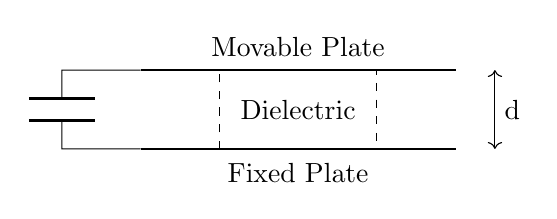
\begin{tikzpicture}
    \draw[thick] (0,0) -- (4,0); \node at (2,-0.3) {Fixed Plate};
    \draw[thick] (0,1) -- (4,1); \node at (2,1.3) {Movable Plate};
    \draw[<->] (4.5,0) -- (4.5,1) node[midway, right] {d};
    \draw[dashed] (1,0) rectangle (3,1); \node at (2,0.5) {Dielectric};
    \draw (0,0) -- (-1,0) to[C] (-1,1) -- (0,1);
\end{tikzpicture}
\captionof{figure}{Capacitive Transducer}
\end{center}

\textbf{Working principle:}
\begin{itemize}
    \item Capacitance $C = \epsilon_0\epsilon_r A/d$
    \item Varies with change in: area (A), distance (d), or dielectric constant ($\epsilon_r$)
    \item Displacement changes the capacitance
\end{itemize}

\textbf{Applications:} Pressure measurement, Liquid level sensing, Humidity sensors, Accelerometers.
\end{solutionbox}

\begin{mnemonicbox}
\mnemonic{CADAP: Capacitance Alters with Distance, Area, or Permittivity.}
\end{mnemonicbox}

\questionmarks{4(c) OR}{7}{Explain LVDT Transducer operation, construction with necessary diagram in detail. Also list advantage, disadvantage and application of LVDT.}

\begin{solutionbox}
LVDT (Linear Variable Differential Transformer) converts linear displacement into electrical output.

\begin{center}
\begin{circuitikz}[american, scale=0.8]
    \draw (0,0) node[inputarrow] {} to[L, l=Pri] (0,2);
    \draw (2, -1) to[L, l=Sec1] (2,0.8);
    \draw (2, 1.2) to[L, l=Sec2] (2,3);
    \draw[thick] (0.5, 0.5) rectangle (1.5, 1.5); \node at (1,1) {Core};
    \draw[<->] (1, 1.6) -- (1, 2.5) node[above] {Displacement};
    \node at (0, -0.5) {AC Input};
    \node at (3, 1) {Output $V_o = V_{s1} - V_{s2}$};
\end{circuitikz}
\captionof{figure}{LVDT}
\end{center}

\textbf{Construction:} Primary coil in center, two secondary coils, movable ferromagnetic core.

\textbf{Operation:}
\begin{itemize}
    \item AC excitation energizes primary coil
    \item Core position determines magnetic coupling to secondaries
    \item Differential voltage output proportional to displacement
\end{itemize}

\textbf{Advantages:} Non-contact, Infinite resolution, High linearity, Robust.

\textbf{Disadvantages:} Requires AC, Bulky, Magnetic sensitivity.

\textbf{Applications:} Precision measurement, Hydraulic systems, Aircraft controls.
\end{solutionbox}

\begin{mnemonicbox}
\mnemonic{CDPOS sensor: Core Displacement Produces Output Signal.}
\end{mnemonicbox}

\questionmarks{5(a)}{3}{Demonstrate working and principle of Semiconductor Temperature Sensor LM35.}

\begin{solutionbox}
LM35 is an IC temperature sensor that outputs voltage linearly proportional to temperature in Celsius.

\begin{center}
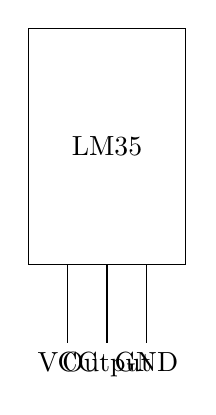
\begin{tikzpicture}
    \draw (0,0) rectangle (2,3);
    \node at (1,1.5) {LM35};
    \draw (0.5,0) -- (0.5,-1) node[below] {VCC};
    \draw (1,0) -- (1,-1) node[below] {Output};
    \draw (1.5,0) -- (1.5,-1) node[below] {GND};
\end{tikzpicture}
\captionof{figure}{LM35 Pinout}
\end{center}

\textbf{Working principle:}
\begin{itemize}
    \item Integrated circuit with built-in temperature-sensing element
    \item Linear output voltage: $+10mV/^\circ$C
    \item Calibrated directly in Celsius
    \item Operating range: -55°C to +150°C
\end{itemize}
\end{solutionbox}

\begin{mnemonicbox}
\mnemonic{TEN mV TRICK: Temperature Escalation Noted in milliVolts: Ten Rise Indicates Celsius Kelvin.}
\end{mnemonicbox}

\questionmarks{5(b)}{4}{Describe working of Harmonic distortion analyzer with necessary diagram.}

\begin{solutionbox}
Harmonic distortion analyzer measures harmonic content to determine signal quality.

\begin{center}
\begin{tikzpicture}[node distance=1.2cm, auto, scale=0.7, every node/.style={transform shape}]
    \node [gtu block] (Input) {Input};
    \node [gtu block, right=of Input] (Atten) {Attenuator};
    \node [gtu block, right=of Atten] (Notch) {Notch Filter};
    \node [gtu block, right=of Notch] (Amp) {Amplifier};
    \node [gtu block, right=of Amp] (RMS) {RMS Detector};
    \node [gtu block, right=of RMS] (Display) {Display};
    
    \draw [gtu arrow] (Input) -- (Atten);
    \draw [gtu arrow] (Atten) -- (Notch);
    \draw [gtu arrow] (Notch) -- (Amp);
    \draw [gtu arrow] (Amp) -- (RMS);
    \draw [gtu arrow] (RMS) -- (Display);
\end{tikzpicture}
\captionof{figure}{Harmonic Distortion Analyzer}
\end{center}

\textbf{Working principle:}
\begin{itemize}
    \item Fundamental frequency filters out using notch filter
    \item Remaining harmonics are measured
    \item THD = (VRMS of harmonics)/(VRMS of fundamental)
\end{itemize}
\end{solutionbox}

\begin{mnemonicbox}
\mnemonic{FRONT analysis: Filter Removes Original Note Totally for Analyzing Leftover Signals.}
\end{mnemonicbox}

\questionmarks{5(c)}{7}{Describe working of Spectrum Analyzer with necessary diagram in detail.}

\begin{solutionbox}
Spectrum Analyzer displays signal amplitude versus frequency.

\begin{center}
\begin{tikzpicture}[node distance=1.2cm, auto, scale=0.7, every node/.style={transform shape}]
    \node [gtu block] (Input) {RF Input};
    \node [gtu block, right=of Input] (Mixer) {Mixer};
    \node [gtu block, right=of Mixer] (IF) {IF Filter};
    \node [gtu block, right=of IF] (Det) {Detector};
    \node [gtu block, right=of Det] (Disp) {Display};
    \node [gtu block, below=of Mixer] (LO) {Local Osc};
    \node [gtu block, below=of Disp] (Sweep) {Sweep Gen};
    
    \draw [gtu arrow] (Input) -- (Mixer);
    \draw [gtu arrow] (Mixer) -- (IF);
    \draw [gtu arrow] (IF) -- (Det);
    \draw [gtu arrow] (Det) -- (Disp);
    \draw [gtu arrow] (LO) -- (Mixer);
    \draw [gtu arrow] (Sweep) -- (LO);
    \draw [gtu arrow] (Sweep) -| (Disp);
\end{tikzpicture}
\captionof{figure}{Spectrum Analyzer}
\end{center}

\textbf{Working principle:}
\begin{itemize}
    \item \textbf{Superheterodyne}: Input mixed with LO
    \item \textbf{Sweep}: LO swept across range
    \item \textbf{Display}: Shows frequency domain spectrum
\end{itemize}

\textbf{Applications:} Signal analysis, EMI testing, Harmonic analysis.
\end{solutionbox}

\begin{mnemonicbox}
\mnemonic{SAFER view: Sweep Analyzes Frequencies for Examining RF.}
\end{mnemonicbox}

\questionmarks{5(a) OR}{3}{Explain analog transducer and digital transducer. Also explain primary transducer and secondary transducer.}

\begin{solutionbox}
\begin{center}
\captionof{table}{Transducer Types}
\begin{tabulary}{\linewidth}{|L|L|}
\hline
\textbf{Type} & \textbf{Description} \\ \hline
\textbf{Analog} & Produces continuous output signal proportional to input \\ \hline
\textbf{Digital} & Produces discrete/binary output signal \\ \hline
\textbf{Primary} & Directly converts physical quantity into electrical/mechanical signal \\ \hline
\textbf{Secondary} & Converts output of primary transducer into another form \\ \hline
\end{tabulary}
\end{center}
\end{solutionbox}

\begin{mnemonicbox}
\mnemonic{PADS: Primary And Digital/analog Secondary.}
\end{mnemonicbox}

\questionmarks{5(b) OR}{4}{Explain working of Digital IC tester with necessary diagram in detail.}

\begin{solutionbox}
Digital IC tester verifies functionality of integrated circuits.

\begin{center}
\begin{tikzpicture}[node distance=1.5cm, auto, scale=0.7, every node/.style={transform shape}]
    \node [gtu block] (Micro) {Microcontroller};
    \node [gtu block, right=of Micro] (Pattern) {Pattern Gen};
    \node [gtu block, right=of Pattern] (Socket) {Test Socket};
    \node [gtu block, below=of Pattern] (Analyzer) {Result Analyzer};
    
    \draw [gtu arrow] (Micro) -- (Pattern);
    \draw [gtu arrow] (Pattern) -- (Socket);
    \draw [gtu arrow] (Socket) |- (Analyzer);
    \draw [gtu arrow] (Analyzer) -| (Micro);
\end{tikzpicture}
\captionof{figure}{Digital IC Tester}
\end{center}

\textbf{Working principle:}
\begin{itemize}
    \item Applies test patterns to IC in socket
    \item Compares output with expected results
    \item Indicates Pass/Fail
\end{itemize}
\end{solutionbox}

\begin{mnemonicbox}
\mnemonic{TRIG test: Test, Run patterns, Identify faults, Generate report.}
\end{mnemonicbox}

\questionmarks{5(c) OR}{7}{Explain working of function generator with necessary diagram in detail.}

\begin{solutionbox}
Function generator produces various waveforms for testing.

\begin{center}
\begin{tikzpicture}[node distance=1.2cm, auto, scale=0.7, every node/.style={transform shape}]
    \node [gtu block] (Freq) {Freq Control};
    \node [gtu block, right=of Freq] (Osc) {Oscillator};
    \node [gtu block, right=of Osc] (Shaper) {Wave Shaper};
    \node [gtu block, right=of Shaper] (Amp) {Amp Control};
    \node [gtu block, right=of Amp] (Out) {Output Amp};
    \node [gtu block, right=of Out] (O) {Output};
    
    \draw [gtu arrow] (Freq) -- (Osc);
    \draw [gtu arrow] (Osc) -- (Shaper);
    \draw [gtu arrow] (Shaper) -- (Amp);
    \draw [gtu arrow] (Amp) -- (Out);
    \draw [gtu arrow] (Out) -- (O);
\end{tikzpicture}
\captionof{figure}{Function Generator}
\end{center}

\textbf{Waveforms:} Sine, Square, Triangle, Ramp.

\textbf{Applications:} Testing amplifiers, Reference signals, Educational demos.
\end{solutionbox}

\begin{mnemonicbox}
\mnemonic{SWATOR: Sine Wave And Triangle OSCillator Renders signals.}
\end{mnemonicbox}

\end{document}
